\documentclass[t]{beamer}
% xcolor and define colors -------------------------
\usepackage[table]{xcolor}

% https://www.viget.com/articles/color-contrast/
\definecolor{purple}{HTML}{5601A4}
\definecolor{navy}{HTML}{0D3D56}
\definecolor{ruby}{HTML}{9a2515}
\definecolor{alice}{HTML}{107895}
\definecolor{daisy}{HTML}{EBC944}
\definecolor{coral}{HTML}{F26D21}
\definecolor{kelly}{HTML}{829356}
\definecolor{cranberry}{HTML}{E64173}
\definecolor{jet}{HTML}{131516}
\definecolor{asher}{HTML}{555F61}
\definecolor{slate}{HTML}{314F4F}

% Mixtape Sessions
\definecolor{picton-blue}{HTML}{00b7ff}
\definecolor{violet-red}{HTML}{ff3881}
\definecolor{sun}{HTML}{ffaf18}
\definecolor{electric-violet}{HTML}{871EFF}

% Main theme colors
\definecolor{accent}{HTML}{00b7ff}
\definecolor{accent2}{HTML}{871EFF}
\definecolor{gray100}{HTML}{f3f4f6}
\definecolor{gray800}{HTML}{1F292D}


% Beamer Options -------------------------------------

% Background
\setbeamercolor{background canvas}{bg = white}

% Change text margins
\setbeamersize{text margin left = 15pt, text margin right = 15pt}

% \alert
\setbeamercolor{alerted text}{fg = accent2}

% Frame title
\setbeamercolor{frametitle}{bg = white, fg = jet}
\setbeamercolor{framesubtitle}{bg = white, fg = accent}
\setbeamerfont{framesubtitle}{size = \small, shape = \itshape}

% Block
\setbeamercolor{block title}{fg = white, bg = accent2}
\setbeamercolor{block body}{fg = gray800, bg = gray100}

% Title page
\setbeamercolor{title}{fg = gray800}
\setbeamercolor{subtitle}{fg = accent}

%% Custom \maketitle and \titlepage
\setbeamertemplate{title page}
{
    %\begin{centering}
        \vspace{20mm}
        {\Large \usebeamerfont{title}\usebeamercolor[fg]{title}\inserttitle}\\
        {\large \itshape \usebeamerfont{subtitle}\usebeamercolor[fg]{subtitle}\insertsubtitle}\\ \vspace{10mm}
        {\insertauthor}\\
        {\color{asher}\small{\insertdate}}\\
    %\end{centering}
}

% Table of Contents
\setbeamercolor{section in toc}{fg = accent!70!jet}
\setbeamercolor{subsection in toc}{fg = jet}

% Button
\setbeamercolor{button}{bg = accent}

% Remove navigation symbols
\setbeamertemplate{navigation symbols}{}

% Table and Figure captions
\setbeamercolor{caption}{fg=jet!70!white}
\setbeamercolor{caption name}{fg=jet}
\setbeamerfont{caption name}{shape = \itshape}

% Bullet points

%% Fix left-margins
\settowidth{\leftmargini}{\usebeamertemplate{itemize item}}
\addtolength{\leftmargini}{\labelsep}

%% enumerate item color
\setbeamercolor{enumerate item}{fg = accent}
\setbeamerfont{enumerate item}{size = \small}
\setbeamertemplate{enumerate item}{\insertenumlabel.}

%% itemize
\setbeamercolor{itemize item}{fg = accent!70!white}
\setbeamerfont{itemize item}{size = \small}
\setbeamertemplate{itemize item}[circle]

%% right arrow for subitems
\setbeamercolor{itemize subitem}{fg = accent!60!white}
\setbeamerfont{itemize subitem}{size = \small}
\setbeamertemplate{itemize subitem}{$\rightarrow$}

\setbeamertemplate{itemize subsubitem}[square]
\setbeamercolor{itemize subsubitem}{fg = jet}
\setbeamerfont{itemize subsubitem}{size = \small}


% Special characters

\usepackage{collectbox}

\makeatletter
\newcommand{\mybox}{%
    \collectbox{%
        \setlength{\fboxsep}{1pt}%
        \fbox{\BOXCONTENT}%
    }%
}
\makeatother





% Links ----------------------------------------------

\usepackage{hyperref}
\hypersetup{
  colorlinks = true,
  linkcolor = accent2,
  filecolor = accent2,
  urlcolor = accent2,
  citecolor = accent2,
}


% Line spacing --------------------------------------
\usepackage{setspace}
\setstretch{1.1}


% \begin{columns} -----------------------------------
\usepackage{multicol}


% Fonts ---------------------------------------------
% Beamer Option to use custom fonts
\usefonttheme{professionalfonts}

% \usepackage[utopia, smallerops, varg]{newtxmath}
% \usepackage{utopia}
\usepackage[sfdefault,light]{roboto}

% Small adjustments to text kerning
\usepackage{microtype}



% Remove annoying over-full box warnings -----------
\vfuzz2pt
\hfuzz2pt


% Table of Contents with Sections
\setbeamerfont{myTOC}{series=\bfseries, size=\Large}
\AtBeginSection[]{
        \frame{
            \frametitle{Roadmap}
            \tableofcontents[current]
        }
    }


% Tables -------------------------------------------
% Tables too big
% \begin{adjustbox}{width = 1.2\textwidth, center}
\usepackage{adjustbox}
\usepackage{array}
\usepackage{threeparttable, booktabs, adjustbox}

% Fix \input with tables
% \input fails when \\ is at end of external .tex file
\makeatletter
\let\input\@@input
\makeatother

% Tables too narrow
% \begin{tabularx}{\linewidth}{cols}
% col-types: X - center, L - left, R -right
% Relative scale: >{\hsize=.8\hsize}X/L/R
\usepackage{tabularx}
\newcolumntype{L}{>{\raggedright\arraybackslash}X}
\newcolumntype{R}{>{\raggedleft\arraybackslash}X}
\newcolumntype{C}{>{\centering\arraybackslash}X}

% Figures

% \imageframe{img_name} -----------------------------
% from https://github.com/mattjetwell/cousteau
\newcommand{\imageframe}[1]{%
    \begin{frame}[plain]
        \begin{tikzpicture}[remember picture, overlay]
            \node[at = (current page.center), xshift = 0cm] (cover) {%
                \includegraphics[keepaspectratio, width=\paperwidth, height=\paperheight]{#1}
            };
        \end{tikzpicture}
    \end{frame}%
}

% subfigures
\usepackage{subfigure}


% Highlight slide -----------------------------------
% \begin{transitionframe} Text \end{transitionframe}
% from paulgp's beamer tips
\newenvironment{transitionframe}{
    \setbeamercolor{background canvas}{bg=accent!40!black}
    \begin{frame}\color{accent!10!white}\LARGE\centering
}{
    \end{frame}
}


% Table Highlighting --------------------------------
% Create top-left and bottom-right markets in tabular cells with a unique matching id and these commands will outline those cells
\usepackage[beamer,customcolors]{hf-tikz}
\usetikzlibrary{calc}
\usetikzlibrary{fit,shapes.misc}

% To set the hypothesis highlighting boxes red.
\newcommand\marktopleft[1]{%
    \tikz[overlay,remember picture]
        \node (marker-#1-a) at (0,1.5ex) {};%
}
\newcommand\markbottomright[1]{%
    \tikz[overlay,remember picture]
        \node (marker-#1-b) at (0,0) {};%
    \tikz[accent!80!jet, ultra thick, overlay, remember picture, inner sep=4pt]
        \node[draw, rectangle, fit=(marker-#1-a.center) (marker-#1-b.center)] {};%
}

\usepackage{math}
\usepackage{verbatim}
\usepackage{bm}
\begin{document}
\imageframe{./lecture_includes/slide_banner.pdf}

\begin{frame}{Two approaches to Modern DID}
  \begin{enumerate}
    \item $2 \times 2$ approach:
    
    \smallskip 
    This approach primarily tries to subset data to a particular set of periods where some units change their treatment and compare to a set of control units that do not change their treatment

    \medskip
    \begin{itemize}
      \item E.g. $\text{ATT}(g, t)$, conditional PTs (outcome regression), continuous DID, units get treated multiple times, etc. 
    \end{itemize}
    

    \pause
    \bigskip
    \item Modelling $Y_{it}(0)$:
    
    \smallskip 
    This approach proposes a model for the untreated potential outcome, estimates that model using $d_{it} = 0$ observations, and `imputes' the missing potential outcome for the $d_{it} = 1$ observations

    \medskip
    \begin{itemize}
      \item E.g. Borusyak et. al. / `did2s', synthetic control, matrix completion / factor model imputation
    \end{itemize}

    
  \end{enumerate}
\end{frame}

\section{Imputation in 2x2}

\begin{frame}{DID Estimator}
  Let's start with our standard DID estimator
  $$
    \expec{Y_{i1} - Y_{i0}}{D_i = 1} - \expec{Y_{i1} - Y_{i0}}{D_i = 0}
  $$

  \bigskip
  \pause
  We can rewrite this in an odd-looking way
  \only<2-3>{
  $$
    \expec{
      Y_{i1} - {\color{electric-violet}
        \left( Y_{i0} + \expec{Y_{i1} - Y_{i0}}{D_i = 0} \right)
      }
    }{D_i = 1}
  $$
  }
  \only<4>{
    $$
      \expec{
        Y_{i1}(1) - \underbrace{\color{electric-violet}
          \left( Y_{i0} + \expec{Y_{i1} - Y_{i0}}{D_i = 0} \right)
        }_{= \hat{Y}_{i1}(0)}
      }{D_i = 1}
    $$
  }

  \bigskip
  \only<3>{
    \begin{itemize}
      \item $\expec{Y_{i1} - Y_{i0}}{D_i = 0}$ is the average change in outcome for control units
      \item Take a treated unit's initial value $Y_{i0}$ and add to it this change in outcome
    \end{itemize}
  }

  \only<4>{
    We are `imputing' missing potential outcome (Imbens, RESTAT 2004)
  }
\end{frame}

\begin{frame}{Imputation}
  $$
    \expec{
      Y_{i1}(1) - \underbrace{\color{electric-violet}
        \left( Y_{i0} + \expec{Y_{i1} - Y_{i0}}{D_i = 0} \right)
      }_{\hat{Y}_{i1}(0)}
    }{D_i = 1}
  $$

  \bigskip
  We can observe untreated PO in the pre-period, but not the post-period.
  \begin{itemize}
    \item We predict how outcome would change using the untreated group
  \end{itemize}

  \pause
  \bigskip
  Identification relies on $\hat{Y}_{i1}(0)$ being a good estimate of $Y_{i1}(0)$ (at least on average)
  \begin{itemize}
    \item This is the parallel (counterfactual) trends assumption
  \end{itemize}
\end{frame}

\begin{frame}{Imputation with Covariates}
  The regression adjustment estimator is also an imputation estimator:

  $$
  \expec{
    Y_{i1}(1) - \underbrace{\color{electric-violet}
      \left( Y_{i0} + \hat{\mu}_{D=0,t=1}(X_i) - \hat{\mu}_{D=0,t=0}(X_i) \right)
    }_{\hat{Y}_{i1}(0)},
  }{D_i = 1}
  $$
  
  \bigskip
  where $\hat{\mu}_{D=0, t}$ is our estimates of $Y_{it}(0)$ given $X_i$ estimated with the untreated units only.
\end{frame}

\begin{frame}{Imputation with Covariates}
  Similarly, the IPW estimator is an imputation estimator but you take a weighted average of
  $$
    \expec{
      Y_{i1}(1) - \underbrace{\color{electric-violet}
        \left(
          Y_{i0} +
          \expec{w_0(X_i) \left( Y_{i1} - Y_{i0} \right)}{D_i = 0}
        \right)
      }_{\hat{Y}_{i1}(0)}
    }{D_i = 1},
  $$
  where $w_0(X_i) = \frac{\hat{p}(X_i)}{1 - \hat{p}(X_i)}$ uses our estimated propensity score 
\end{frame}


\section{Imputation with Staggered Treatment Timing}

\begin{frame}{TWFE Model}

  Unit $i$ at time $t$ has outcome $y_{it}$ given by the TWFE model with heterogeneous effects:

  $$
  y_{it} = \mu_i + \eta_t + \tau_{it} d_{it} + \varepsilon_{it},
  $$
  with $\expec{\varepsilon_{it}} = 0$. $\eta_t$ are common time shocks, $\mu_i$ are unit-specific time-invariant shocks.
  
  \bigskip
  $d_{it}$ is a treatment dummy for being actively under treatment.
  Units can vary in what year they get treated.
\end{frame}

\begin{frame}{TWFE Model}{Treatment effect heterogeneity}
  \begin{center}
    $\tau_{it}$ in most settings is heterogeneous
  \end{center}

  \bigskip
  Treatment effects may depend on when you start treatment
  \begin{itemize}
    \item \emph{e.g.}, groups that benefit more from a policy implement it earlier
  \end{itemize}

  \bigskip
  Treatment effects may depend on treatment duration (event study!)
  \begin{itemize}
    \item \emph{e.g.}, policy doesn't affect everyone right away
  \end{itemize}
\end{frame}

\begin{frame}{Ignoring heterogeneous effects}

  Say we ignore $\tau_{it}$ and simplify our model to

  $$
    y_{it} = \mu_i + \eta_t + \tau d_{it} + \underbrace{u_{it}}_{ \varepsilon_{it} + (\tau_{it} - \tau) d_{it} }
  $$

  \medskip
  The error term now contains the treatment effect heterogeneity.
  \begin{itemize}
    \item If there is any systematic heterogeneity like we described before, then the covariates (unit and time indicators) are correlated with the error term and OLS estimates suffer from omitted variables bias.
  \end{itemize}
\end{frame}

\begin{frame}{Estimating overall average treatment effect}
  If we knew $\mu_i$ and $\eta_t$, then we could move terms around in our model:
  $$
  y_{it} - \mu_i - \eta_t = \tau_{it} d_{it} + \varepsilon_{it}
  $$

  \pause
  \bigskip
  If we regress $y_{it} - \mu_i - \eta_t$ on the dummy variable $d_{it}$, OLS algebra tells us that $\hat{\tau}$ will estimate a simple average of $\tau_{it}$ (plus noise):

  $$
    \hat{\tau} = \frac{1}{N_{\text{post}}} \sum_{(i,t) \ : \ d_{it} = 1} \left( \tau_{it} d_{it} + \varepsilon_{it} \right) = \text{ATT} + \text{noise},
  $$
  % where $N_{\text{post}}$ is the number of post-treatment observations
\end{frame}

\begin{frame}{Estimating dynamic ATTs}
  Similarly, if we had a set of \emph{mutually-exclusive} event-study dummy variables, $d_{it}^\ell$, and run
  
  $$
    y_{it} - \mu_i - \eta_t = \sum_{\ell} \tau^\ell_{it} d_{it}^\ell + u_{it}
  $$
  \bigskip
  we would get averages of $\tau_{it}$ for $(i,t)$ with $g_i - t = \ell$.
\end{frame}

\begin{frame}{Too bad we don't know $\mu$ and $\eta$}

  Since we don't know $\mu$ and $\eta$, we have to estimate them. Using the FWL theorem our OLS estimate is equivalent to:
  $$
    y_{it} - \hat{\mu}_i - \hat{\eta}_t = \tau \tilde{d}_{it} + u_{it},
  $$

  where $\tilde{d}_{it}$ is the \emph{residualized} treatment dummy.
\end{frame}

\begin{frame}{Using OLS to estimate $\mu$ and $\eta$}
  $$
    y_{it} - \hat{\mu}_i - \hat{\eta}_t = \tau \tilde{d}_{it} + u_{it},
  $$

  \bigskip
  All of the modern diff-in-diff problems (yes all of them) show different ways to interpret the same problem: $\tilde{d}_{it}$.
  \begin{itemize}
    \item Since we have residualized $\tilde{d}_{it}$, not the indicator $d_{it}$, OLS no longer computes the simple average of $\tau_{it}$'s.
  \end{itemize}
\end{frame}

\begin{frame}{Fixing the problem}
  $$
  y_{it} - \hat{\mu}_i - \hat{\eta}_t = \tau_{it} \tilde{d}_{it} + u_{it},
  $$

  \bigskip
  Okay, so why don't you just regress $y_{it} - \hat{\mu}_i - \hat{\eta}_t$ on $d_{it}$? \pause Great intuition!
\end{frame}

\begin{frame}{Two-stage difference-in-differences}
  Proposed in concurrent work by Borusyak et. al. (2024) and Gardner (2021). I adopt the nomenclature of Gardner (2021).

  \bigskip
  \textbf{Stage 1:}
  Estimate $\mu_i$ and $\eta_t$ using untreated/not-yet-treated observations ($d_{it} = 0$).
  \begin{itemize}
    \item Don't include $d_{it} = 1$ obs. since the treatment effects will bias estimates of the fixed effects.
  \end{itemize}

  \pause
  \bigskip
  \textbf{Stage 2:}
  Regress $Y_{it} - \underbrace{\left( \hat{\mu}_i + \hat{\eta}_t \right)}_{\hat{Y}_{it}(0)}$ on $d_{it}$.
\end{frame}

\begin{frame}{Inference}
  \textbf{Stage 2:}
  Regress $Y_{it} - \underbrace{\left( \hat{\mu}_i + \hat{\eta}_t \right)}_{\hat{Y}_{it}(0)}$ on $d_{it}$.

  \bigskip
  Inference is complicated because the outcome variable in the second-stage is a `generated regressor'.
  \begin{itemize}
    \item Inference is taken care for you in \texttt{did2s} (or you can block bootstrap!)
  \end{itemize}
\end{frame}

\begin{frame}{Pseudocode}
  \textbf{R Code:}
  \medskip

  \texttt{library(fixest)}

  \texttt{fs = feols(y $\sim$ 0 | unit + time, data = df[df\$d == 0, ])}

  \texttt{df\$y\_resid = df\$y - predict(fs, newdata = df)}

  \texttt{ss = feols(y\_resid $\sim$ d, data = df)}


  \bigskip\bigskip
  \textbf{Stata Code:}
  \medskip

  \texttt{reg y i.unit i.time if d == 0}

  \texttt{predict y0\_hat, xb}

  \texttt{gen y\_resid = y - y0\_hat}

  \texttt{reg y0\_hat i.d}
\end{frame}

\begin{frame}{Imputation Extensions}
  For this very simple TWFE model, imputation is just a (yet another) way of estimating staggered DIDs
  \begin{itemize}
    \item But, the procedure generalizes in a lot of ways that prove useful
  \end{itemize}
\end{frame}

\begin{frame}{Essential ingredient \#1}{Model for $Y_{it}(0)$}
  \begin{enumerate}
    \item Posit an explicit model for $Y_{it}(0)$
    \begin{itemize}
      \item this can include time-interacted covariates, linear time-trends, etc.
      
      \item in your paper, you get to write down a very explicit model for outcomes
    \end{itemize}
  \end{enumerate}

  Our parallel trends assumption comes in that our fitted model is an unbiased estimator for $Y_{it}(0)$ in the post-treatment periods \emph{for the treated units}.
  \begin{itemize}
    \item E.g. our time fixed-effects are fit using the control group in the post-periods. Need these to be the same time effects as the treated group.
  \end{itemize}
\end{frame}

\begin{frame}{Essential ingredient \#2}{Estimation and imputation}
  \begin{enumerate}
    \setcounter{enumi}{1}
    \item Estimate that model using observations that are not impacted by treatment ($d_{it} = 0$) and then impute missing counterfactual for $d_{it} = 1$
    \begin{itemize}
      \item You have in your dataset both the observed $Y_{it} = Y_{it}(1)$ and the imputed $\hat{Y}_{it}(0)$ (like in a synthetic control plot)
    \end{itemize}
  \end{enumerate}
\end{frame}

\begin{frame}{Essential ingredient \#3}{Averaging treatment effects}
  \begin{enumerate}
    \setcounter{enumi}{2}
    \item Take $Y_{it} - \hat{Y}_{it}(0)$ and average it however you wish to aggregate effects
    \begin{itemize}
      \item Overall ATT, dynamic event-study, event-study separately by some characteristic (e.g. by gender) 
    \end{itemize}
  \end{enumerate}
\end{frame}


\subsection{Stacking}

\begin{frame}{Stacking}
  I think the usefulness of the imputation procedure really shows itself in `more advanced treatment' settings.

  \bigskip
  For example, Cengiz, Dube, Lindner, and Zipperer (QJE, 2019) think about state-level minimum wage changes.
  \begin{itemize}
    \item Problem: Not a binary absorbing treatment since states change minimum wage more than once.

    \item But there are few enough minimum wage changes, there should be a valid control group that can be used.
  \end{itemize}
\end{frame}

\begin{frame}{Minimum Wage Example Continued.}
  \bigskip
  For each minimum wage change (an `event'), the authors create a filtered dataset and run a DID on the subset
  \begin{itemize}
    \item Treated counties and a set of `clean control states' that did not have a minimum wage change within 4 years of the `event'
    \item Subset to $\pm 4$ years from event
  \end{itemize}
\end{frame}

\imageframe{lecture_includes/dube_event_by_event.png}

\begin{frame}{Stacked overall estimate}
  They, then want to estimate an `overall' estimate by pooling across events. To do so they `stack' the dataset (\texttt{dplyr::bind\_rows} or \texttt{append using} in a for loop) and then run the following event-study regression:
  $$
    Y_{e,it} = \mu_{e,i} + \eta_{e,t} + \sum_{\ell} \tau^\ell d_{it}^\ell + u_{e,it},
  $$
  where $e$ denotes the event-dataset $e$.
  \begin{itemize}
    \item Note the treatment dummies are not interacted with $e$ so we estimate an overall average effect
  \end{itemize}
\end{frame}

\begin{frame}{Stacking Pros and Cons}
  I think the stacking approach is popular because:
  \begin{itemize}
    \item Tailor the control group to a `good' set of control units (e.g. bordering counties, matching counties with similar $X$, etc.).
    \begin{itemize}
      \item All the other packages use all the control units for every treated group by default (there are workarounds)
    \end{itemize}

    \item You write an explicit model for $Y_{it}(0)$
  \end{itemize}

  \bigskip
  But it comes with some costs:
  \begin{itemize}
    \item Annoying and error-prone; interacting a bunch of terms; bunch of for loops; make sure you filter dataset right; hard to write up and hard to read; etc.
    \item Identifies a convex-average of $\tau_{it}$ but the weights are non-standard and data-dependent (e.g. can change by adding more pre-periods)
  \end{itemize}
\end{frame}

\begin{frame}{Imputation and Stacking}
  In a new WIP (by me), make this procedure much simpler (using the imputation strategy):

  \bigskip
  \textbf{First Stage:}

  For each event, $e$,
  \begin{itemize}
    \item Fit model of $Y_{it}(0)$ using the pre-treatment observations and the `clean controls' for that event.

    \item For event-$e$ treated units, impute their post-$e$ outcomes.
  \end{itemize}

  \bigskip
  \textbf{Second Stage:}

  Regress $Y_{it} - \hat{Y}_{it}(0)$ on $d_{it}$ or $d_{it}^\ell$.


  \bigskip\bigskip
  {\tiny \emph{Sigh}. I started this last year before Codechella and haven't even touched it yet. I had to prep 3 classes this year, we were hiring for 4 positions this year, I published my JMP, and I'm really tired}
\end{frame}

\begin{frame}{Imputation and Stacking}
  Advantages include:
  \begin{itemize}
    \item Identify $ATT$ (not a weirdly weighted average)
    \item Inference is easy
    \item Easy to write-up: For each event, here is our model of $Y_{it}(0)$ and here are the control units we use
  \end{itemize}
\end{frame}

\begin{frame}{Imputation Estimators}
  Imputation estimators offer a few benefits:
  \begin{itemize}
    \item They allow you to transparently write down your model for the untreated potential outcome and estimate that model
    \item They naturally adapt to more complex models for $Y_{it}(0)$ beyond the two-way fixed effect model (next sections)
  \end{itemize}
\end{frame}

\section{Modeling non-parallel trends}

\begin{frame}{Covariates and Conditional PTs}
  Let $i$ denote workers and $t$ denote the year. $X_i$ be the amount of schooling the worker has.

  \bigskip
  A general model for wages might look like:
  $$
    w_{it}(0) = \mu_i + \eta_t + g_t(X_i)+ u_{it},
  $$
  where $g_t(X_i)$ changes over time and causes non-parallel trends. Conditional parallel-trends implies that $\expec{u_{it}} = 0$.

  \bigskip
  Comparing two units with the same $X_i = x$, then $g_t(x)$ is the same for those units receive the same time shocks $\eta_t + g_t(x)$.
  \begin{itemize}
    \item This is the essence of conditional parallel-trends.
  \end{itemize}
\end{frame}

\begin{frame}{Covariates and Conditional PTs}
  A common choice is $g_t(X_i) = X_i \beta_t$

  \begin{itemize}
    \item Trends are caused by changing returns to characteristic $X_i$, $\beta_{t} - \beta_{t-1}$.

    % \item Can estimate $\beta_t$ by interacting $X_i$ with time-dummies.

    \item Linearity is the default for \texttt{did}/\texttt{DRDID} Sant'Anna and Zhao implementation

    \pause
    \item Linearity is strong. In a period, going from 8 to 9 years of schooling has the same increase in wages as 14 to 15 years. Maybe you think the profile is non-linear (e.g. quadratic)
  \end{itemize}

  \bigskip\pause
  Could make more flexible with polynomials like $X_i \beta_{1,t} + X_i^2 \beta_{2,t}$ or by binning $X_i$ and interacting with time.
\end{frame}

\begin{frame}{Covariate-specific trends and non-PTs}
  Let's go with the linear model:
  $$
    w_{it}(0) = \mu_i + \eta_t + X_i \beta_t + u_{it},
  $$

  \pause
  Say you don't include $X_i$ in your regression, when would this create a problem?

  $$
    \expec{w_{i1} - w_{i0}}{D_i = d} =
      \left( \eta_1 - \eta_0 \right) +
      \expec{X_i}{D_i = d} \left( \beta_1 - \beta_0 \right)
  $$
  \begin{itemize}
    \item In the linear case, if treated and control units don't have different average values of $X_i$, then unconditional PTs hold

    \item Conversely, if units enter treatment based on $X_i$, then non-parallel trends is induced.
    % \item With more general $g_t(X_i)$ case, need distribution of $X_i$ to not vary by treatment.
  \end{itemize}
\end{frame}

\begin{frame}{Non-observed covariates}
  In the worker's wage example, we might suspect that something like computer-skill might be unobservable and have a time-varying impact.

  \bigskip That is both $X_i$ and $\beta_t$ are unobserved!

  \begin{itemize}
    \item If the job-training program attracts people with more computer-skills (e.g. excel workshop), then PTs does not hold.
    \item We can not `compare two individuals with the same value of $X_i$' since we do not observe them.
  \end{itemize}
\end{frame}


\begin{frame}{(Linear) Factor Models}
  We've just walked through the motivation for a `factor model', sometimes called `interactive-fixed effects model'.

  \bigskip
  There are a set of $\rho$ unit characteristics $\lambda_{i,r}$ and a set of corresponding time-specific shocks $f_{t, r}$ whose impact on $Y$ is given by:
  $$
    Y_{it} = \sum_{r=1}^\rho \lambda_{i, r} f_{t, r} + \varepsilon_{it}
  $$

  \begin{itemize}
    \item Same logic as before, $\lambda_i$ measures the unit's characteristic and $f_{t,r}$ is the shock to returns of the characteristic.

    \pause
    \item This nests the two-way fixed effects model $f_t = 1$ implies unit fixed-effects, $\lambda_i = 1$ implies time fixed-effects
  \end{itemize}
\end{frame}

\begin{frame}{(Linear) Factor Models}
  $$
    Y_{it} = \sum_{r=1}^\rho \lambda_{i, r} f_{t, r} + \varepsilon_{it}
  $$

  \bigskip
  Let's give an example using county-level aggregate employment.
  \begin{itemize}
    \item $\lambda_i$ might consist of (i) manufacturing share and (ii) share of college-educated
    \item In each period, shocks to the national economy change manufacturing demand and (ii) technological change drives returns to college degree
  \end{itemize}

  \pause
  \bigskip
  We might have ideas of what are the primary characteristics are, but we might not have data on it. If you do, then we are back in $X_i$ land.
\end{frame}

\begin{frame}{Imputation and (Linear) Factor Models}
  We have a more-general model for $Y_{it}(0)$ now that allows some forms of non-parallel-trends:
  $$
    Y_{it}(0) =  \mu_i + \eta_t + \sum_{r=1}^\rho \lambda_{i, r} f_{t, r} + \varepsilon_{it}
  $$

  \bigskip\bigskip
  Can we estimate this and use our imputation procedure?
  \begin{itemize}
    \item The short-answer is yes. There is a bunch of different approaches but they're not as simple as TWFE.

    \item The factor model is much more data-hungry than fixed effects, usually requiring both a large number of units \emph{ and } a large number of time-periods.
  \end{itemize}
\end{frame}





\section{Synthetic Control}

\begin{frame}{Synthetic Control}
  The standard synthetic control method considers a single treated unit (country, state, firm, etc.). We will let $\bm{Y}_i = \left( Y_{i1}, \dots, Y_{iT} \right)'$ be the vector of outcomes for unit $i$. The treated unit is $i = 0$.

  \bigskip\pause
  Synthetic control imputes $\bm{Y}_0(0)$ for the treated unit using a weighted average of the control units:
  $$
    \hat{\bm{Y}}_0(0) = \sum_{i = 1}^N w_i \bm{Y}_i
  $$
  \begin{itemize}
    \item Take a part of this state, a part of that state, and then average them together into a `synthetic control' unit
    \item In most cases, we use convex weights $1 \geq w_i \geq 0$.
  \end{itemize}
\end{frame}


\begin{frame}{Choosing weights}
  We wnat our synthetic control unit to do a good job at approximating the pathway of outcomes for the treated unit: $\bm{Y}_0(0)$.

  \pause
  \bigskip
  We only observe $Y_{0t}(0)$ for the treated unit up until period $T_0$ which is the period prior to treatment.
  \begin{itemize}
    \item Synthetic control should try to match the treated unit's outcome path during the pre-period and \emph{HOPEFULLY} that will mean the synthetic control will do a good job in the post-period. It's a leap of faith
  \end{itemize}
\end{frame}

\begin{frame}{Choosing weights}
  More formally, the weights are selected by trying to minimize the following:
  $$
    \argmin_{ \{ w_i \} } \sum_{t=1}^{T_0} \left( Y_{0t} - \sum_{i=1}^N w_i Y_{it} \right)^2
  $$
  \begin{itemize}
    \item Minimizing the pre-treatment sum of squared prediction errors between treated unit and the synthetic control unit.
    \item With convex weights, $1 \geq w_i \geq 0$, we add these as a constrained optimization problem
    % \item Sometimes pre-treatment covariates are used and squared error is summed across the covariates
  \end{itemize}
\end{frame}


\begin{frame}{Example: California's Proposition 99}
	In 1988, California first passed comprehensive tobacco control legislation:
  \begin{itemize}
		\item increased cigarette tax by 25 cents/pack
		\item earmarked tax revenues to health and anti-smoking budgets
		\item funded anti-smoking media campaigns
		\item spurred clean-air ordinances throughout the state
		\item produced more than \$100 million per year in anti-tobacco projects
  \end{itemize}

  \bigskip Other states that subsequently passed control programs are excluded from donor pool of controls (AK, AZ, FL, HI, MA, MD, MI, NJ, OR, WA, DC)
\end{frame}

% \begin{frame}{Cigarette Consumption: CA and the Rest of the US}
\imageframe{./lecture_includes/abadie_3.pdf}
% \end{frame}

% \begin{frame}{Cigarette Consumption: CA and synthetic CA}
\imageframe{./lecture_includes/abadie_4.pdf}
% \end{frame}

% \begin{frame}{Sparsity and Synthetic Control Weights}
\imageframe{./lecture_includes/synth_smoking_table2.png}
% \end{frame}


\begin{frame}{\emph{Beware of Overfitting}}
  Intuitively, synthetic control is `believable' when the synthetic control unit does a great job at approximating the outcome in the per-period
  \begin{itemize}
    \item We think that the synthetic control must be picking up on underlying economic structure in order to co-move with the treated state.
    \item E.g. if you see a set of runners whose times go up and go down during the same races, you might think they train together. You wouldn't think that chance alone made them have the same ups and downs.
  \end{itemize}

  \pause
  \bigskip
  The number one concern you should have when reading or writing a paper that uses a synthetic control method is that of overfitting.
  \begin{itemize}
    \item If I have 1000 control units and 4 pre-periods, I can probably well approximate $Y_{0t}$ in the pre-period by just random chance.
  \end{itemize}
\end{frame}

\begin{frame}{Synthetic Control and Factor Model}
  Recall our factor model:
  \begin{itemize}
    \item There are a set of characteristics that the units have and in each period a set of macroeconmic shocks that change the marginal effect of those characteristics
    \item If we could observe these characteristics, we would want to match on them or use them in conditional PTs
  \end{itemize}

  \pause
  \bigskip
  Synthetic control, under conditions we will discuss, will create a synthetic control unit that has the same average characteristics as the treated unit!
  \begin{itemize}
    \item Since they are subject to the shocks the same amount, we think their outcome evolutions will match.
  \end{itemize}
\end{frame}

\begin{frame}{Synthetic Control and Factor Model}
  Okay, so I've pained a very rosy picture of synthetic control. When it works well, we fix the problem of non-parallel trends and we are able to impute the untreated potential outcome well.

  \bigskip
  However, I want to make clear that this method is \textbf{not a panacea}. The original paper is very general and makes it hard to know when it works and when it does not.
  \begin{itemize}
    \item More recent advancements all base discussion on a factor model for outcomes
    \item Hollingsworth and Wing working paper has great discussion
  \end{itemize}
\end{frame}

\begin{frame}{Bias of Synthetic Control}
  The original Abadie, Diamond and Hainmueller paper derive the bias of synthetic control when outcomes are generated by a linear factor-model.

  \bigskip
  The bias arises from \textbf{over-fitting on noise}. It is more common to over-fit on data when:
  \begin{itemize}
    \item There are fewer pre-treatment periods $T_0$

    \item There are many control units

    \item The `convex hull' assumption is unlikely to ˙old
  \end{itemize}
\end{frame}

\begin{frame}{`Convex Hull' Assumption}
  When constraining the weights to be convex ($0 \leq w_i \leq 1$), the synthetic control assumption requires the `convex hull' assumption:
  \begin{itemize}
    \item This is basically an assumption that says `we can approximate $\bm{Y}_{0}$ using a convex weighted average of control $\bm{Y}_i$'
  \end{itemize}

  \pause
  \bigskip
  With a factor model, we can make this assumption a lot clearer:
  \begin{itemize}
    \item The `convex hull' assumption is equivalent to the assumption that the treated unit's `factor loadings' are a convex average of the other units' `factor loadings'
    \begin{itemize}
      \item That is, the treated unit can not have an extreme value in any of the $\lambda_{i,r}$ (e.g. huge manufacturing share)
    \end{itemize}
  \end{itemize}
\end{frame}

\begin{frame}{Inference in Synthetic Control}
  Inference in the classical synthetic control setting is really difficult
  \begin{itemize}
    \item Only one treated unit; you're not averaging over units so the estimate is subject to random shocks
  \end{itemize}

  \pause
  \bigskip
  Two forms of randomization inference are typically used:
  \begin{itemize}
    \item Randomly shuffle treatment to control units and reestimate synthetic control; want the treated unit to look more extreme than the placebo estimates. The so-called `spaghetti plot'

    \item Randomly shuffle time-periods around for treated unit and reestimate synthetic control
  \end{itemize}
\end{frame}

\begin{frame}{Implementing Synthetic Control}
  My recommendation for synthetic control is \texttt{scpi} package (on R, Stata, and Python)
  \begin{itemize}
    \item Covers all the basic method and include inference methods

    \item Journal of Statistical Software paper is super readable: \url{https://nppackages.github.io/references/Cattaneo-Feng-Palomba-Titiunik_2024_JSS.pdf}
  \end{itemize}

\end{frame}


\section{More General Factor Model Imputation}

\begin{frame}{`Extensions' of the Synthetic Control Model}{Synthetic Control with Lasso/Ridge Penalty}
  People seem to like when the synthetic control is made up of a few units
  \begin{itemize}
    \item Makes the control unit more `interpretable'
  \end{itemize}
\end{frame}

\begin{frame}{`Extensions' of the Synthetic Control Model}{Synthetic Control with Lasso/Ridge Penalty}
  Can modify the weights optimization problem to penalize weights being too large:
  $$
    \argmin_{ \{ w_i \} } \sum_{t=1}^{T_0} \left( Y_{0t} - \sum_{i=1}^N w_i Y_{it} \right)^2 + \lambda \| w \|_k
  $$
  \begin{itemize}
    \item Add a term that punishes when weights are non-zero; $\lambda$ is a `tuning-parameter' to chose how much to punish
    \item Can add convex-weights constraint
    \item Lasso is $k = 1$; Ridge is $k = 2$
  \end{itemize}
\end{frame}


\begin{frame}{`Extensions' of the Synthetic Control Model}{Augmented Synthetic Control}
  Augmented control is a method to help with imperfect pre-treatment fit by estimating a bias and subtracting it off.
  \begin{itemize}
    \item Looks similar to regression adjustment (DRDID without weights). We estimate the trend using covariates and then use that model to bias correct.
  \end{itemize}
\end{frame}

\begin{frame}{`Extensions' of the Synthetic Control Model}{Augmented Synthetic Control}
  \begin{enumerate}
    \item Calculate the standard synthetic control method weights (or with lasso)
    \item Estimate a model of $m_{t}(X_i) = \expec{\bm{Y}_{it}}{X_i}$ using untreated units where $X_i$ is pre-treatment characteristics (lagged $Y$ or covariates)
  \end{enumerate}

  \bigskip
  Form synthetic control estimate as
  $$
    \left( Y_{0t} - \sum_{i = 1}^N w_i Y_{it} \right) -
      \underbrace{\left( m_{t}(X_0) - \sum_{i = 1}^N w_i m_t(X_i) \right)}_{\text{`bias correction'}}
  $$
\end{frame}



\begin{frame}{`Extensions' of the Synthetic Control Model}{Synthetic Difference-in-Differences}
  Synthetic Control is based on the idea of `finding control units that follow the same fluctuations as the treated unit in the pre-period'
  \begin{itemize}
    \item Some periods are more informative than others (typically more recent years), so we should prefer to fit on those
  \end{itemize}

  This
\end{frame}



\begin{frame}{Example Synthetic DID}
  \begin{columns}[T]
    \begin{column}{.65\textwidth}
      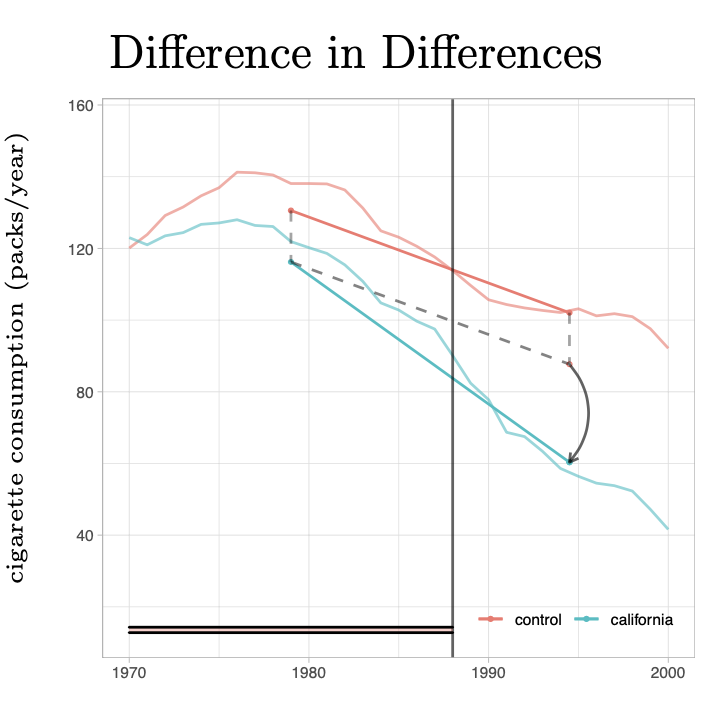
\includegraphics[width=\textwidth]{lecture_includes/sdid_2.png}
    \end{column}
    \hfill
    \begin{column}{.3\textwidth}
      Estimated decrease: -27.3 (17.7)
    \end{column}
  \end{columns}
\end{frame}

\begin{frame}{Example Synthetic DID}
  \begin{columns}[T]
    \begin{column}{.65\textwidth}
      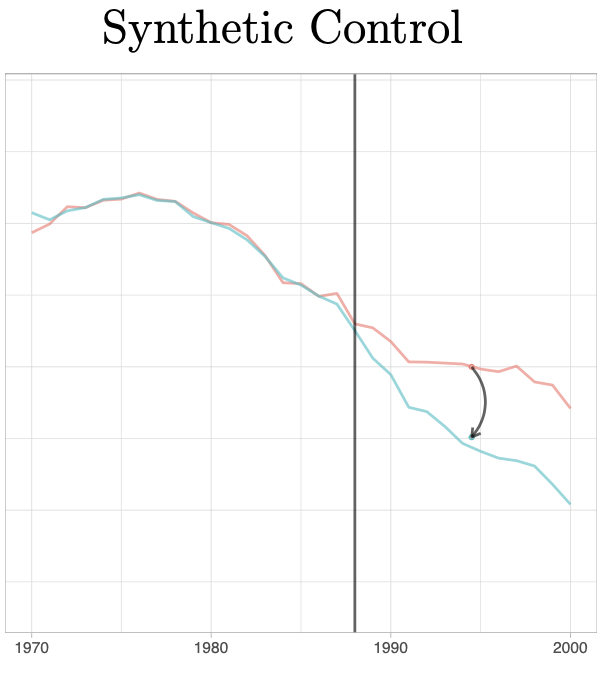
\includegraphics[width=\textwidth]{lecture_includes/sdid_1.png}
    \end{column}
    \hfill
    \begin{column}{.3\textwidth}
      Estimated decrease: -19.6 (9.9)

      \bigskip Bad fit just prior because all time periods are weighted equally
    \end{column}
  \end{columns}
\end{frame}

\begin{columns}[T]
  \begin{column}{.65\textwidth}
    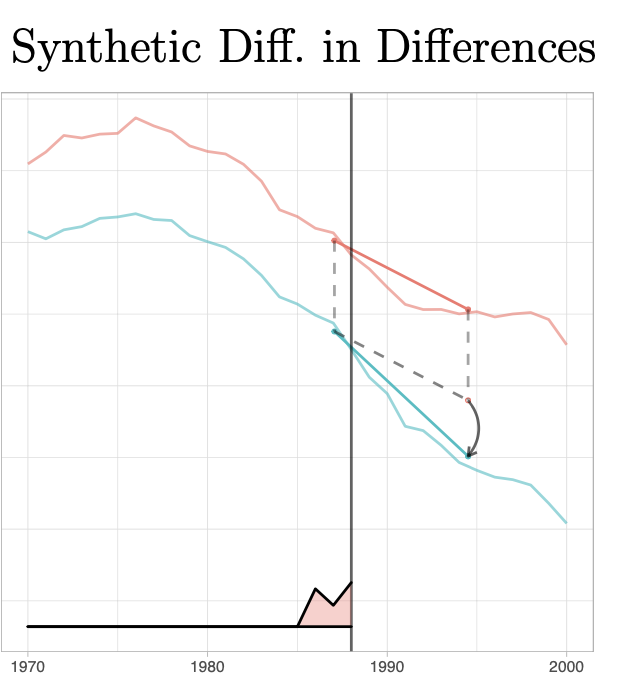
\includegraphics[width=\textwidth]{lecture_includes/sdid_3.png}
  \end{column}
  \hfill
  \begin{column}{.3\textwidth}
    Estimated decrease: -19.6 (9.9)

    \bigskip Most weights on most recent years
  \end{column}
\end{columns}


\begin{frame}{`Extensions' of the Synthetic Control Model}{Generalized Imputation Estimator}
  Xu (2017) and Gobillon and Magnac (2016) both answer a simple question:
  \begin{itemize}
    \item Why not just estimate the factor model directly and impute untreated potential outcomes?
  \end{itemize}

  \bigskip
  Intuition is to estimate $\lambda_{i,r}$ and $f_{t,r}$ using untreated/not-yet-treated observations and then impute:
  $$
    \hat{Y}_{it}(0) = \hat{\mu}_i + \hat{\lambda}_t + \sum_{r=1}^\rho \hat{\lambda}_{i, r} \hat{f}_{t, r}
  $$
  \begin{itemize}
    \item We estimate the non-parallel trending via the factor model and then subtract it off
  \end{itemize}
\end{frame}

\begin{frame}{Factor Model Imputation}
  Unlike imputation of the two-way fixed effect model, this approach is very data hungry:
  \begin{itemize}
    \item Requires both a large number of time-periods and units
  \end{itemize}

  \bigskip
  Intuitively, you need a long number of time-periods to estimate a unit's $\lambda_{i,r}$. You need a large number of units to estimate a time-period's $f_{t,r}$

  \pause
  \bigskip
  This estimator is likely more efficient when the underlying model is a factor model, but biased if a different underlying model is true
  \begin{itemize}
    \item E.g. a non-linear factor model
  \end{itemize}
\end{frame}

\begin{frame}{Problem with large-$T$}
  These new tools are all really powerful, but all rely on having access to many years of data.
  In a lot of applied work, the data is just not available

  \pause
  \bigskip
  But I think there is a more subtle problem at play with this assumption:
  \begin{itemize}
    \item Data from many years ago might not be very useful at understanding the underlying confounders at play in this economy
    \item Imagine saying "I use data from 1960 to inform me which counties would be a good control group for housing prices in 2000". A lot has happened since then !!!!!!
  \end{itemize}
\end{frame}

\begin{frame}{Small-$T$ methods}
  There is a nascent literature thinking about adapting factor-model estimators in settings with very few pre-periods available:
  \begin{itemize}
    \item Basically (1) my work with Nicholas Brown and (2) work by Brantly Callaway and coauthors
  \end{itemize}

  \bigskip
  To conclude today, I'll discuss briefly my work
  \begin{itemize}
    \item But, it's been a long workshop, so I'll keep the self-promo short :-)
  \end{itemize}
\end{frame}

\begin{frame}{Small-$T$ methods}
  It turns out that estimation of treatment effects in short panels with a large number of treated units only requires estimation of $f_{t,r}$
  \begin{itemize}
    \item The only reason we needed large panels was to estimate $\lambda_{i, r}$, so we can do estimation in $f_{t,r}$
  \end{itemize}

  \pause
  \bigskip
  We develop a general approach to impuation in short panels that sounds a lot like the two-way fixed effects version:
  \begin{enumerate}
    \item Using just the untreated group, estimate $f_{t,r}$
    \item Perform imputation of outcome variable (in paper)
    \item Take averages of $Y_{it} - \hat{Y}_{it}(0)$
  \end{enumerate}

  I'll discuss two main aproaches to estimate $f_{t,r}$ in short-panels
\end{frame}

\begin{frame}{Estimation of $f_{t,r}$}{Instrument Approach}
  We've discussed quite a bit during this workshop on thinking about the underlying characteristics that we think could cause non-parallel trends
  \begin{itemize}
    \item This is the same thought exercise as chosing covariates $X_i$
  \end{itemize}

  \pause
  \bigskip
  In some cases, you might be able to form some \emph{noisy} measure of the exposure variables $\lambda_{i,r}$ (e.g. baseline value of share of college educated). These can be used as an instrumental variable to estimate $f_{t,r}$
  \begin{itemize}
    \item The relevancy condition is that $\lambda_{i,r}$ is correlated with the instrument
  \end{itemize}
\end{frame}

\begin{frame}{Estimation of $f_{t,r}$}{Time-varying covariates approach}
  Alternatively, we might have a set of time-varying covariates, $w_{it}$ that we think are impacted by the same macroeconomic shocks $f_{t,r}$ that impacts the outcome variable

  \begin{itemize}
    \item In this case, we can learn about the underlying shocks by movements in $w_{it}$
  \end{itemize}
\end{frame}

\begin{frame}{Factor Models}
  I think factor models are a really great tool for an applied econometrician
  \begin{itemize}
    \item We often want to study treatment in panel settings where we know treated units are selected
    \item But, if we think the treated units are on different trends based on broad macroeconomic shocks (and not location-specific shocks), then a factor model can estimate these broad trends and remove them from biasing our estimates
  \end{itemize}

  \bigskip
  A lot of these estimators require long panels to estimate treatment effects consistently
  \begin{itemize}
    \item We have discussed why even long panels might be undesirable
  \end{itemize}
\end{frame}

\end{document}
